\documentclass[a4paper]{article}
%%%%% TODO:
%%%%% use actual style, fix prelude to conform
\usepackage{tikz}

\usepackage{filecontents}
\usepackage{pgfplots, pgfplotstable}
\usepgfplotslibrary{statistics}

\usepackage[T1]{fontenc}
\usepackage[utf8]{inputenc}

\usepackage{tablefootnote}

%\usepackage{color}
\usepackage{hyperref}

%\usepackage{subcaption}

\usepackage[round,sectionbib]{natbib}
%% https://tex.stackexchange.com/questions/148992/changing-the-heading-style-of-references-section
%% and jfp1.cls
\renewcommand\refname{References}
\makeatletter
\renewcommand\bibsection{%
  \section*{\refname}%
}%
\makeatother

\usepackage{csquotes}

% \usepackage{placeins} %% unneeded

\usepackage{microtype}
\DisableLigatures[>,<]{encoding = T1,family=tt*} 

% für Listings
%\usepackage{listings}


\renewcommand{\cite}[1]{\citep{#1}}

\newcommand{\citHughes}{\citep{HughesArrows}}

%\newcommand{\inlinecode}[1]{\texttt{#1}}
\newcommand{\inlinecode}[1]{\emph{#1}} %%% booo
%%% |code| is inline code in lhs2tex

%\newcommand{\fixme}[1]{\colorbox{red}{#1}}

%%%%%% more fun and typography

\usepackage{xifthen}

\newboolean{anonymous}
\setboolean{anonymous}{False}

\usepackage[british]{babel}

\usepackage{siunitx}

%%\usepackage{tipa} %% causes problems with lhs2tex?!

\usepackage{xspace}
\usepackage{xcolor}
\newcommand{\hl}[1]{\textcolor{red}{#1}}
\newcommand{\comm}[2]{\textcolor{red}{\bfseries #1: #2}}
%\newcommand{\comm}[2]{}
\newcommand{\olcomment}[1]{\comm{OL}{#1}}
\newcommand{\mbcomment}[1]{\comm{MB}{#1}}
\newcommand{\ptcomment}[1]{\comm{Phil}{#1}}
%\newcommand{\done}{\xspace\hl{done!}\xspace}
\newcommand{\fixme}{\mbcomment}

%\renewcommand{\olcomment}[1]{}
%\renewcommand{\mbcomment}[1]{}

\DeclareRobustCommand{\xth}{\textsuperscript{th}\xspace}
\DeclareRobustCommand{\st}{\textsuperscript{st}\xspace}
\DeclareRobustCommand{\nd}{\textsuperscript{nd}\xspace}
\DeclareRobustCommand{\xrd}{\textsuperscript{rd}\xspace}

%% kuerzel
%\newcommand{\todo}{\textcolor{red}{\bfseries TODO!}\xspace}
\newcommand{\done}{\textcolor{green}{\bfseries done!}\xspace}
\DeclareRobustCommand{\hairspn}{\hspace{1pt}\nolinebreak}% hair space with no break

\newcommand{\seconds}{~s}

% \DeclareRobustCommand{\ie}{{i.\hairspn{}e.\nopagebreak[4] }}
% \DeclareRobustCommand{\eg}{{e.\hairspn{}g.\nopagebreak[4] }}
% \DeclareRobustCommand{\fe}{{f.\hairspn{}e.,}\nopagebreak[4] }
\DeclareRobustCommand{\ie}{{i.\hairspn{}e.~}}
\DeclareRobustCommand{\eg}{{e.\hairspn{}g.~}}
\DeclareRobustCommand{\fe}{{f.\hairspn{}e.,~}}
\DeclareRobustCommand{\ad}{{A.\hairspn{}D.\xspace}}
\DeclareRobustCommand{\bcc}{{A.\hairspn{}C.\xspace}}
\DeclareRobustCommand{\wrt}{w.\hairspn{}r.\hairspn{}t.~}
\DeclareRobustCommand{\etc}{etc.\ }
\DeclareRobustCommand{\cf}{\textit{cf.~}}
\DeclareRobustCommand{\viz}{\textit{viz.~}}
%\DeclareRobustCommand{\hof}{higher-or\-der function\xspace}

% %% the numberings
\DeclareRobustCommand{\xth}{\textsuperscript{th}\xspace}
\DeclareRobustCommand{\st}{\textsuperscript{st}\xspace}
\DeclareRobustCommand{\nd}{\textsuperscript{nd}\xspace}
\DeclareRobustCommand{\xrd}{\textsuperscript{rd}\xspace}

\newcommand{\tabsepbakup}{\tabcolsep}
%% for narrower tables

%% nice tables
\usepackage{booktabs}
%\usepackage{multirow}

%% more microtype
\microtypecontext{spacing=nonfrench} %% log said so

\usepackage{subfig}


%% fight for pipepipepipe
\newcommand{\pipepipepipe}{\ensuremath{\mathbin{\mid\!\mid\!\mid}}\xspace}
%%% ^^^^ keep consistent with definition at the top of main.lhs
%%%\newcommand{\pipepipepipe}{\inlinecode{|||}\xspace}

%%% JFP requirements:
%%% Harvard citing style, "(Curry 1933)".
%%% code: identifies italic, keywords bold
%%% figures: eps(!) or ps (can convert pdf), eventually provide a greyscale version, color NOT in cmyk

\usepackage[T1]{fontenc}
\usepackage{lmodern}

\title{Arrows for Parallel Computations}
\date{\today}
\ifthenelse{\boolean{anonymous}}{%
\author{Submission ID xxxxxx}
}{%
\author{Martin Braun, Phil Trinder, and Oleg Lobachev}
%\affiliation{University Bayreuth, Germany and Glasgow University, UK}
}

\begin{document}	
        \maketitle
	%
	\begin{abstract}
Arrows form\olcomment{are?} a general interface for computation and pose therefore as an alternative to monads for API design. We express parallelism using this concept. This is a new way to represent parallel computation. We define an Arrows-based interface for parallelism and implement it using multiple parallel Haskells.
\olcomment{Benefits:} In this manner we are able to bridge across various parallel Haskells with a common interface.

This new way of writing parallel programs has a benefit of being portable across flavours of parallel Haskells.\olcomment{Wdh?}
Each parallel computation is an arrow, they can be composed and transformed as such.
We thus introduce some syntactic sugar to provide parallelism-aware arrow combinators.

We also define  several parallel skeletons with our framework. 
Benchmarks shows that our framework does not induce too much overhead performance-wise.
\end{abstract}
	%
	%\newpage
	\tableofcontents
	%\pagebreak
	%\section{Motivation}
%Arrows were introduced in John Hughes paper as a general interface for computation and therefore as an alternative to Monads for API design \citHughes. In the paper Hughes describes how arrows are a generalization of Monads and how they are not as restrictive. In this paper we will use this concept to express parallelism.

\section{Introduction}
\label{sec:introduction}
% \olcomment{todo, reuse 5.5, and more}
%
% \mbcomment{
% Haskell is Spielwiese für Parallelität; verschiedene Ansätze (Par, Multicore, Eden); Orthogonale Ansätze; Verwenden höchstens eine Monade - manchmal auch nur intern; Wir wollen Parallelität mit Arrows abbilden, was noch niemand gemacht hat;
% Statt einer eigenen Implementierung definieren wir ein "shallow embedded DSL" (ACHTUNG, ist das der richtige Name? effektiv API);
% Umsetzung mit verschiedenen parallelen Haskells; We tame the zoo of parallel Haskells und vergewissern uns dass es nicht viel Overhead bringt
% }
%
% blablabla arrows, parallel, haskell.
%
% \olcomment{An attempt ---->}
%%%%%

Parallel functional languages have a long history of being used for experimenting with novel parallel programming paradigms including the expression of parallelism. Haskell, which we focus on in this paper, has  several mature implementations. We regard here in-depth
Glasgow parallel Haskell or short GpH (its Multicore SMP implementation, in particular), the
|Par| Monad, and Eden, a distributed memory parallel Haskell. These
languages represent orthogonal approaches. Some use a monad, even if
only for the internal representation. Some introduce additional
language constructs. Section \ref{sec:parallelHaskells} gives a short overview over these languages.

%In this paper we introduce a notion of parallel
%computations using Arrows.
A key novelty in this paper is to use Arrows to represent parallel computations. They seem a natural fit as they are a generalization of the function arrow (|->|) and serve as general interface to computations. Section \ref{sec:arrows} gives a short introduction to Arrows.

%Our Arrows-based interface is a high-level one.
We provide an Arrows-based type class and implementations for the three above mentioned parallel Haskells.
Instead of 
introducing a new low-level parallel backend in order to implement our
Arrows-based interface, we define a shallow-embedded DSL for Arrows. This DSL
is defined as a common interface with varying implementations in
the existing parallel Haskells. Thus, we not only define a parallel programming interface in a
novel manner - we tame the zoo of parallel Haskells. We provide a
common \ptcomment{quantify, e.g. less than 10 \%} \mbcomment{we do this in the contributions section of the Introduction, enough?}, very low-penalty programming interface that allows to switch
the parallel backends at will. The induced penalty was max. 8.3 \% in our measurements. Further backends based on HdpH or a Frege implementation (on the Java Virtual Machine) are viable, too.

\paragraph{Contributions}
%
%\olcomment{HIT HERE REALLY STRONG}
%
%\subsection{Impact of parallel Arrows}
%\olcomment{move this to Contributions in the front or something}
We propose a new Arrow-based encoding for parallelism based on a new Arrow combinator |parEvalN :: [arr a b] -> arr [a] [b]| in Section \ref{sec:parallel-arrows}, which converts a list of Arrows into a new parallel Arrow. A parallel Arrow is still an Arrow, hence the resulting parallel Arrow can still be used in the same way as a potential sequential version.

We evaluate the expressive power of Arrow formalism in the context of parallel programming.

\begin{itemize}
\item We introduce a parallel evaluation formalism using Arrows. One big advantage is that we do not introduce any new types (Sec.~\ref{sec:parallel-arrows}) in contrast Monad solutions such as |Par| Monad. This behaviour encourages better composability.
\item We utilitze multiple backends -- currently a GpH, a |Par| Monad, and Eden. We do not reimplement all the parallel internals, as we host this functionality in the |ArrowParallel| type class, which abstracts all parallel implementation logic. The backends can easily be swapped, so we are not bound to any specific one.

So as an example, during development, we can run the program in a simple GHC-compiled variant using a GpH backend and afterwards deploy it on a cluster by converting it into an Eden program, by just replacing the |ArrowParallel| instance and compiling with Eden's GHC variant. (Sec.~\ref{sec:parallel-arrows})
\item We extend our PArrows formalism with |Future|s. Our goal here is to enable direct communication of data between nodes in a distributed memory setting similar to Eden's Remote Data (|RD|). Direct communication is useful in a distributed memory setting because they allow for inter-node communication without blocking the master-node. (Sec.~\ref{sec:futures})
\item It is possible to define algorithmic skeletons with PArrows (Sec.~\ref{sec:skeletons})
\item Finally, we demonstrate that Arrow parallelism is a viable alternative to existing approaches. It introduces only low overhead (Sec.~\ref{sec:benchmarks}).
\end{itemize}

\mbcomment{Überleitung auf Related Work hier machen}



\mbcomment{Mention Future work here?}

\mbcomment{Conclusion?}

%\ptcomment{* We evaluate the expressive power of  arrow parallelism. Showing that 
%  + there is no need to introduce additional types
%  + that it is possible to define algorthmic skeletons (Section 6,7)
%  + ...

%* We demonstrate that Arrow Parallelism can exploit multiple parallel %Haskell implementations, and with low overhead, i.e. less than X%. 
%... (Section 8) }

%We wrap parallel Haskells inside of our |ArrowParallel| typeclass, but
% why do we aim to abstract parallelism this way and what does this
% approach do better than the other parallel Haskells?
% is such a parallelism abstraction of benefit and to what extent does
% it improve existing approaches?
%\begin{itemize}
%	\item \textbf{Arrow DSL benefits}:
%    To implement parallelism, we do not introduce any new types, but only rely on a typeclass that hosts |parEvalN :: [arr a b] -> arr [a] [b]|, which converts a list of arrows into a new parallel arrow. Therefore, we do not lose any benefits of using arrows as parallelism is just encapsulated in yet another Arrow combinator. The resulting Arrow can be used in the same way a potential serial version could be used. This is a big advantage of this approach, especially compared to Monad solutions like the |Par| Monad which require specialized Monad types. We can just \enquote{plug} in parallel parts into sequential Arrow-based programs without having to change anything.
%	\item \textbf{Abstraction}:
%	With the |ArrowParallel| typeclass, we abstract all parallel implementation logic away from the business logic. This means it is possible to write code against the interface of a common typeclass without being bound to any parallel Haskell. So as an example, during development, we can run the program in a simple GHC-compiled variant and afterwards deploy it on a cluster by converting it into an Eden version, by just replacing the current |ArrowParallel| instance.
%\end{itemize}


%\paragraph{Structure}
%The remaining text is structures as follows. Section~\ref{sec:background} briefly introduces known parallel Haskell flavours (Sec.~\ref{sec:parEvalNIntro}) and gives an overview of Arrows to the reader (Sec.~\ref{sec:arrows}). Section~\ref{sec:related-work} discusses related work. Section~\ref{sec:parallel-arrows} defines Parallel Arrows and presents a basic interface. Section~\ref{futures} defines Futures for Parallel Arrows, this concept enables better communication. Section~\ref{sec:map-skeletons} presents some basic algorithmic skeletons  in our newly defined dialect: parallel |map| with and without load balancing. More advanced skeletons are showcased in Section~\ref{sec:topology-skeletons} (|pipe|, |ring|, |torus|). Section~\ref{sec:benchmarks} shows the benchmark results. Section~\ref{sec:conclusion} discusses future work and concludes.

%%% Local Variables:
%%% mode: latex
%%% TeX-master: "main"
%%% End:

	\section{Introduction to parallel Haskells}

\begin{lstlisting}[frame=htrbl]
parEvalN :: [a -> b] -> [a] -> [b]
\end{lstlisting}

\frbreak

\subsection{Multicore Haskell}
\begin{lstlisting}[frame=htrbl]
parEvalN :: (NFData b) => [a -> b] -> [a] -> [b]
parEvalN fs as = zipWith ($) fs as `using` parList rdeepseq
\end{lstlisting}

\frbreak

\subsection{ParMonad}
\begin{lstlisting}[frame=htrbl]
parEvalN :: (NFData b) => [a -> b] -> [a] -> [b]
parEvalN fs as = runPar $ 
(sequenceA $ map (spawnP) $ zipWith ($) fs as) >>= mapM get
\end{lstlisting}

\frbreak

\subsection{Eden}
\begin{lstlisting}[frame=htrbl]
parEvalN :: (Trans a, Trans b) => [a -> b] -> [a] -> [b]
parEvalN fs as = spawnF fs as
\end{lstlisting}
	%\pagebreak
	\section{Related Work}
\label{sec:related-work}
\olcomment{todo}



%%% Local Variables:
%%% mode: latex
%%% TeX-master: "main"
%%% End:

	\section{Arrows}
Arrows were introduced by Hughes \citHughes ~as a general interface for computation. An arrow \code{arr a b} can be look at as a computation that converts an input \code{a} to an output \code{b}. This is defined in the arrow typeclass:
\begin{lstlisting}[frame=htrbl]
class Arrow arr where
	arr :: (a -> b) -> arr a b
	(>>>) :: arr a b -> arr b c -> arr a c
	first :: arr a b -> arr (a,c) (b,c)
\end{lstlisting}
\lstinline{arr} is used to lift an ordinary function to an arrow type. This can be thought of as analogous to the monadic \lstinline{return}. The \lstinline{>>>} operator, in a similar way, is analogous to the monadic composition operator \lstinline{>>=} and combines two arrows \code{arr a b} and \code{arr b c} by "wiring" the outputs of the first to the inputs to the second to get a new arrow \code{arr a c}. And lastly, the \lstinline{first} operator, which takes the input arrow from b to c and converts it into an arrow on pairs with the second argument untouched, is also needed for actual useful code as without it, we wouldn't have a way to save input across arrows.
\\\\
The most prominent instances of this interface are regular functions \lstinline{(->)},
\begin{lstlisting}[frame=htrbl]
instance Arrow (->) where
	arr f = f
	f >>> g = g . f
	first f = \(a, c) -> (f a, c) 
\end{lstlisting}
and the Kleisli type.
\begin{lstlisting}[frame=htrbl]
instance Arrow (Kleisli m) where
	arr f = Kleisli $ return . f
	f >>> g = Kleisli $ \a -> f a >>= g
	first f = Kleisli $ \(a,c) -> f a >>= \b -> return (b,c)
\end{lstlisting}
With this typeclass in place, Hughes also defined some syntactic sugar: The mirrored version of \lstinline{first}, called \lstinline{second},
\begin{lstlisting}[frame=htrbl]
second :: Arrow arr => arr a b -> arr (c, a) (c, b)
second f = arr swap >>> first f >>> arr swap
	where swap (x, y) = (y, x)
\end{lstlisting}
the *** combinator which combines first and second to handle two inputs in one arrow,
\begin{lstlisting}[frame=htrbl]
(***) :: Arrow arr => arr a b -> arr c d -> arr (a, c) (b, d)
f *** g = first f >>> second g
\end{lstlisting}
and the \&\&\& combinator that constructs an arrow which outputs 2 different values like ***, but takes only one input.
\begin{lstlisting}[frame=htrbl]
(&&&) :: Arrow arr => arr a b -> arr a c -> a a (b, c)
f &&& g = arr (\a -> (a, a)) >>> (f *** g)
\end{lstlisting}
A short example given by Hughes on how to use this is \lstinline{add} over arrows:
\begin{lstlisting}[frame=htrbl]
add :: Arrow arr => arr a Int -> arr a Int -> arr a Int
add f g = (f &&& g) >>> arr (\(u, v) -> u + v)
\end{lstlisting}
The benefit of using the \code{Arrow} typeclass is that any type which is shown to be an arrow can be used in conjunction with this newly created \lstinline{add} combinator. Even though this example is quite simple, the power of the arrow interface immediately is clear: If a type is an arrow, it can immediately used together with every library that works on arrows. Compared to simple monads, this enables us to write code that is more extensible, without touching the internals of the specific arrows.
\\\\
\textit{Note: In the definitions Hughes gave in his paper, the notation \code{a b c} for an arrow from \code{b} to \code{c} is used. We use the equivalent definition \code{arr a b} for an arrow from \code{a} to \code{b} instead, to make it easier to find the arrow type in type signatures. We kept the original notation \code{a b c} for this section to not change too much from Hughes' original definitions.}
	%\pagebreak
	%\pagebreak
	\subsection{Generalization to Arrows}


\begin{frame}[fragile]{The ArrowParallel typeclass}
\begin{lstlisting}[frame=htrbl]
parEvalN :: [a -> b] -> [a] -> [b]
\end{lstlisting}

\begin{lstlisting}[frame=htrbl]
parEvalN :: (Arrow arr) => [arr a b] -> arr [a] [b]
\end{lstlisting}

\begin{lstlisting}[frame=htrbl]
class Arrow arr => ArrowParallel arr a b where
	parEvalN :: [arr a b] -> arr [a] [b]
\end{lstlisting}
\begin{lstlisting}[frame=htrbl]
class Arrow arr => ArrowParallel arr a b conf where
	parEvalN :: conf -> [arr a b] -> arr [a] [b]
\end{lstlisting}

\end{frame}

	%\pagebreak
	\section{Basic Skeletons}

With the \code{ArrowParallel} typeclass in place and implemented, we can now implement some basic parallel skeletons.

\subsection{parEvalNLazy}
\begin{center}
	\includegraphics[scale=0.7]{images/parEvalNLazy}
\end{center}
\code{parEvalN} is 100\% strict, which means that it fully evaluates all passed arrows. Sometimes this might not be feasible, as it will not work on infinite lists of functions like e.g. \code{map (arr . (+)) [1..]} or just because we need the arrows evaluated in chunks. \code{parEvalNLazy} fixes this. It works by first chunking the input from \code{[a]} to \code{[[a]]} with the given \code{ChunkSize} in \code{arr (chunksOf chunkSize)}. These chunks are then fed into a list \code{[arr [a] [b]]} of parallel arrows created by feeding chunks of the passed \code{ChunkSize} into the regular parEvalN by using \code{listApp}. The resulting \code{[[b]]} is lastly converted into \code{[b]} with \code{arr concat}.
\begin{lstlisting}[frame=htrbl]
parEvalNLazy :: (ArrowParallel arr a b conf, ArrowChoice arr, ArrowApply arr) =>
	conf -> ChunkSize -> [arr a b] -> (arr [a] [b])
parEvalNLazy conf chunkSize fs =
	arr (chunksOf chunkSize) >>>
	listApp fchunks >>>
	arr concat
	where
		fchunks = map (parEvalN conf) $ chunksOf chunkSize fs
\end{lstlisting}

\subsection{parEval2}
\begin{center}
	\includegraphics[scale=0.7]{images/parEval2}
\end{center}
We have only talked about the paralellization arrows of the same type until now. But sometimes we want to paralellize heterogenous types as well. However, we can implement such a \code{parEval2} combinator which combines two arrows \code{arr a b} and \code{arr c d} into a new parallel arrow \code{arr (a, c) (b, d)} quite easily with the help of the \code{ArrowChoice} typeclass. The idea is to use the \code{+++} combinator which combines two arrows \code{arr a b} and \code{arr c d} and transforms them into \code{arr (Either a c) (Either b d)} to get a common arrow type that we can then feed into parEvalN.
\\\\
We start by transforming the \code{(a, c)} input into a 2-element list \code{[Either a c]} by first tagging the two inputs with \code{Left} and \code{Right} and wrapping the right element in a singleton list with \code{return} so that we can combine them with \code{arr (uncurry (:))}. Next, we feed this list into a parallel arrow running on 2 instances of \code{f +++ g} as described above. After the calculation is finished we convert the resulting \code{[Either b d]} into \code{([b], [d])} with \code{arr partitionEithers}. The two lists in this tuple contain only 1 element each by construction, so we can finally just convert the tuple to \code{(b, d)} in the last step.
\begin{lstlisting}[frame=htrbl]
parEval2 :: (ArrowChoice arr,
	ArrowParallel arr (Either a c) (Either b d) conf) =>
	conf -> arr a b -> arr c d -> arr (a, c) (b, d)
parEval2 conf f g = 
	arr Left *** (arr Right >>> arr return) >>>
	arr (uncurry (:)) >>>
	parEvalN conf (replicate 2 (f +++ g)) >>>
	arr partitionEithers >>>
	arr head *** arr head
\end{lstlisting}
	%\pagebreak
	\section{Syntactic Sugar} \label{syntacticSugar}
For basic arrows, we have the \code{***} combinator which allows us to combine two arrows \code{arr a b} and \code{arr c d} into an arrow \code{arr (a, c) (b, d)} which does both computations at once. This can easily be translated into a parallel version with \code{parEval2}, but for this we require a backend which has an implementation that does not require any configuration (hence the \code{()} as the conf parameter in the following code snippet).
\begin{lstlisting}[frame=htrbl]
(|***|) :: (ArrowChoice arr, ArrowParallel arr (Either a c) (Either b d) ())) =>
	arr a b -> arr c d -> arr (a, c) (b, d)
(|***|) = parEval2 ()
\end{lstlisting}
With this we can analogously to the serial \code{&&&} define the parallel \code{|&&&|}.
\begin{lstlisting}[frame=htrbl]
(|&&&|) :: (ArrowChoice arr, ArrowParallel arr (Either a a) (Either b c) ()) =>
	arr a b -> arr a c -> arr a (b, c)
(|&&&|) f g = (arr $ \a -> (a, a)) >>> f |***| g
\end{lstlisting}
	%\pagebreak
	\subsection{Futures}
\begin{frame}[fragile]{without Futures}
\begin{lstlisting}[frame=htrbl]
someCombinator :: [arr a b] -> [arr b c] -> arr [a] [c]
someCombinator fs1 fs2 =
	parEvalN () fs1 >>>	rightRotate >>>	parEvalN () fs2
\end{lstlisting}
\pause
\begin{center}
\includegraphics[scale=0.3]{images/withoutFutures}
\end{center}
\end{frame}
\begin{frame}[fragile]{Future definition}
Since the particular concepts and implementations differ from backend to backend, we define the Future typeclass:
\begin{lstlisting}[frame=htrbl]
class Future fut a conf | a conf -> fut where
    put :: (Arrow arr) => conf -> arr a (fut a)
    get :: (Arrow arr) => conf -> arr (fut a) a
\end{lstlisting}
\end{frame}
\begin{frame}[fragile]{Future implementation (Eden)}
\begin{lstlisting}[frame=htrbl]
data RemoteData a = RD { rd :: RD a }

put' :: (Arrow arr) => arr a (BasicFuture a)
put' = arr BF

get' :: (Arrow arr) => arr (BasicFuture a) a
get' = arr (\(~(BF a)) -> a)

instance NFData (RemoteData a) where
    rnf = rnf . rd
instance Trans (RemoteData a)

instance (Trans a) => Future RemoteData a Conf where
    put _ = put'
    get _ = get'
\end{lstlisting}
\end{frame}
\begin{frame}[fragile]{with Futures}
\begin{lstlisting}[frame=htrbl]
someCombinator :: [arr a b] -> [arr b c] -> arr [a] [c]
someCombinator fs1 fs2 =
	parEvalN () (map (>>> put ()) fs1) >>>
	rightRotate >>>
	parEvalN () (map (get () >>>) fs2)
\end{lstlisting}
\pause
\begin{center}
\includegraphics[scale=0.35]{images/withFutures}
\end{center}
\end{frame}
	%\pagebreak
	\section{Skeletons}
\label{sec:skeletons}
Now we have developed Parallel Arrows far enough to define some useful algorithmic skeletons that abstract typical parallel computations. While there are many possible skeletons to implement, we demonstrate the expressive power of PArrows here using four |map|-based and three toplogical skeletons.
%%% \FloatBarrier
\subsection{|map|-based Skeletons}
\label{sec:map-skeletons}
The essential differences between the mapping skeletons presented here are in terms of order of evaluation and work distribution but still provide the same semantics as a sequential |map|.

\paragraph{Parallel |map| and laziness.}
The |parMap| skeleton (Figs.~\ref{fig:parMapImg},~\ref{fig:parMap}) is probably the most common skeleton for parallel programs. We can implement it with |ArrowParallel| by repeating an Arrow |arr a b| and then passing it into |parEvalN| to obtain an Arrow |arr [a] [b]|.
Just like |parEvalN|, |parMap| traverses all input Arrows as well as the inputs.
Because of this, it has the same restrictions as |parEvalN| as compared to |parEvalNLazy|. So it makes sense to also have a |parMapStream| (Figs.~\ref{fig:parMapStreamImg},~\ref{fig:parMapStream}) which behaves like |parMap|, but uses |parEvalNLazy| instead of |parEvalN|. Implementing these skeletons is straightforward as in Appendix \ref{app:omitted} in Figs.\ref{fig:parMap} and \ref{fig:parMapStream}.

\begin{figure}[thb]
%farm
\includegraphics[scale=0.7]{images/farm}
\caption{|farm| depiction.}
\label{fig:farmImg}

\begin{code}
farm :: (ArrowParallel arr a b conf,
	ArrowParallel arr [a] [b] conf, ArrowChoice arr) =>
	conf -> NumCores -> arr a b -> arr [a] [b]
farm conf numCores f =
	unshuffle numCores >>>
	parEvalN conf (repeat (mapArr f)) >>>
	shuffle
\end{code}
\caption{|farm| definition.}
\label{fig:farm}

%farmChunk
\includegraphics[scale=0.7]{images/farmChunk}
\caption{|farmChunk| depiction.}
\label{fig:farmChunkImg}
\end{figure}

\paragraph{Statically load-balancing parallel |map|.}
Our |parMap| spawns every single computation in a new thread (at least for the instances of |ArrowParallel| we presented in this paper). This can be quite wasteful and a statically load-balancing |farm| (Figs.~\ref{fig:farmImg},~\ref{fig:farm}) that equally distributes the workload over |numCores| workers seems useful.
The definitions of the helper functions |unshuffle|, |takeEach|, |shuffle| (Fig.~\ref{fig:edenshuffleetc}) originate from an Eden skeleton\footnote{Available on Hackage under \url{https://hackage.haskell.org/package/edenskel-2.1.0.0/docs/src/Control-Parallel-Eden-Map.html}.}.

%\paragraph{Lazy statically load-balancing parallel map}
Since a |farm|  is basically just |parMap| with a different work distribution, it has the same restrictions as |parEvalN| and |parMap|. We can, however, define |farmChunk| (Figs.~\ref{fig:farmChunkImg},~\ref{fig:farmChunk}) which uses |parEvalNLazy| instead of |parEvalN|. It is basically the same definition as for |farm|, but with |parEvalNLazy| instead of |parEvalN|.

%%% Local Variables:
%%% mode: latex
%%% TeX-master: "main"
%%% End:

	%\pagebreak
	\section{Topology Skeletons}
Even though many algorithms can be expressed by parallel maps, some problems require more sophisticated skeletons. The Eden library leverages this problem and already comes with more predefined skeletons, among them are a \code{pipe}, \code{ring} and a \code{torus} implementation \cite{eden_cefp, eden_skel_topology}. These seem like reasonable candidates to be ported to our arrow based parallel Haskell to prove that we can express such skeletons with Arrows as well.

\subsection{pipe}

The parallel pipe skeleton is semantically equivalent to folding over a list \code{[arr a a]} of arrows with \code{>>>}, but does this in parallel, meaning that the arrows don't have to reside on the same thread/machine. We implement this skeleton using the \code{ArrowLoop} typeclass which enables us to use \code{loop :: arr (a, b) (c, b) -> arr a c}.

\begin{lstlisting}[frame=htrbl]
pipeSimple :: (ArrowLoop arr, ArrowParallel arr a a conf) =>
	conf -> [arr a a] -> arr a a
pipeSimple conf fs =
	loop (arr snd &&& (arr (uncurry (:) >>> lazy) >>>
		parEvalN conf fs)) >>>
	arr last
\end{lstlisting}
where \code{lazy} is defined as:
\begin{lstlisting}[frame=htrbl]
lazy :: (Arrow arr) => arr [a] [a]
lazy = arr (\ ~(x:xs) -> x : lazy xs)
\end{lstlisting}
However, using this definition directly, will result in the master node becoming a potential bottleneck in distributed environments as described in chapter \ref{futures}. Therefore, a more sophisticated version that uses Futures internally is a good idea:
\begin{lstlisting}[frame=htrbl]
pipe :: (ArrowLoop arr, ArrowParallel arr (fut a) (fut a) conf,
	Future fut a) =>
	conf -> [arr a a] -> arr a a
pipe conf fs = unliftFut (pipeSimple conf (map liftFut fs))
\end{lstlisting}
Sometimes, this pipe definition can be a bit inconvenient, especially if we want to pipe arrows of mixed types together, i.e. \code{arr a b} and \code{arr b c}. By wrapping these two arrows inside a common type
\begin{lstlisting}[frame=htrbl]
pipe2 :: (ArrowLoop arr, ArrowChoice arr,
	ArrowParallel arr (fut (([a], [b]), [c])) (fut (([a], [b]), [c])) conf,
	Future fut (([a], [b]), [c])) =>
	conf -> arr a b -> arr b c -> arr a c
pipe2 conf f g = 
	(arr return &&& arr (const [])) &&& arr (const []) >>>
	pipe conf (replicate 2 (unify f g)) >>>
	arr snd >>>
	arr head
		where
			unify :: (ArrowChoice arr) =>
				arr a b -> arr b c -> arr (([a], [b]), [c]) (([a], [b]), [c])
			unify f g =
				(mapArr f *** mapArr g) *** arr (\_ -> []) >>>
				arr (\((a, b), c) -> ((c, a), b))
\end{lstlisting}
Note that extensive use of this combinator over \code{pipe} with a hand-written combination data-type will probably result in worse performance because of more communication overhead from the many calls to parEvalN. Nonetheless, we can define a parallel piping operator \code{|>>>|} which is semantically equivalent to \code{>>>} similar to the other parallel syntactic sugar from chapter \ref{syntacticSugar}:
\begin{lstlisting}[frame=htrbl]
(|>>>|) :: (ArrowLoop arr, ArrowChoice arr,
	ArrowParallel arr (fut (([a], [b]), [c])) (fut (([a], [b]), [c])) (),
	Future fut (([a], [b]), [c])) =>
	arr a b -> arr b c -> arr a c
(|>>>|) = pipe2 ()
\end{lstlisting}

\subsection{ring}
Eden's ring implementation allows a ring of functions to communicate over direct channels. We can rewrite its functionality easily again with the use of \code{loop}. In each loop we start by rotating the intermediary input from the nodes \code{[fut r]} with \code{second (rightRotate >>> lazy)}. We have to feed the intermediary input into \code{lazy} or the evaluation would hang. The reasoning was explained by \cite{eden_cefp}:
\begin{quotation}
Note that the list of ring inputs ringIns is the same as the list of ring outputs ringOuts rotated by one element to the right using the auxiliary function rightRotate. Thus, the program would get stuck without the lazy pattern, because the ring input will only be produced after process creation and process creation will not occur without the first input.
\end{quotation}
Next, we zip the resulting \code{([i], [fut r])} to \code{[(i, fut r)]} with \code{arr (uncurry zip)} so we can feed that into a our input arrow \code{arr (i, r) (o, r)}, which we transform into \code{arr (i, fut r) (o, fut r)} before lifting it to \code{arr [(i, fut r)] [(o, fut r)]} to get a list \code{[(o, fut r)]}. Finally we unzip this list into \code{([o], [fut r])}. Plugging this arrow \code{arr ([i], [fut r]) ([o], fut r)} into the definition of \code{loop} from earlier gives us \code{arr [i] [o]}, our ring arrow.
\begin{center}
	\includegraphics[scale=0.75]{images/ring}
\end{center}
\begin{lstlisting}[frame=htrbl]
ring :: (ArrowLoop arr, Future fut r,
	ArrowParallel arr (i, fut r) (o, fut r) conf) =>
    conf ->
    arr (i, r) (o, r) ->
    arr [i] [o]
ring conf f =
	loop (second (rightRotate >>> lazy) >>>
    arr (uncurry zip) >>>
    parMap conf (second get >>> f >>> second put) >>>
    arr unzip)
\end{lstlisting}
with \code{rightRotate}:
\begin{lstlisting}[frame=htrbl]
rightRotate :: (Arrow arr) => arr [a] [a]
rightRotate = arr $ \list -> case
	list of [] -> []
			xs -> last xs : init xs
\end{lstlisting}
and lazy:
\begin{lstlisting}[frame=htrbl]			
lazy :: (Arrow arr) => arr [a] [a]
lazy = arr (\ ~(x:xs) -> x : lazy xs
\end{lstlisting}
This combinator can be used for example to calculate the shortest paths in a graph using Warshall's algorithm. Further details on this can be found in \cite{eden_cefp}.
\subsection{torus}
\begin{center}
	\includegraphics[scale=0.75]{images/torus}
\end{center}
If we take the concept of a ring one dimension further, we get a torus. Every node sends ands receives data from horizontal and vertical neighbours in each communication round. This gives us . With our parallel Arrows we implement a torus combinator yet again with the help of the \code{ArrowLoop} typeclass.
\\\\
Inside the loop we once again start by rotating the input, but this time not only in one direction, but in two. This means that the intermediary input from the neighbour nodes has to be stored in a tuple \code{([[fut a]], [[fut b]])} in the second argument (loop only allows for 2 arguments) of our input \code{([[c]], ([[fut a]], [[fut b]]))} and our rotation arrow becomes \code{second ((mapArr rightRotate >>> lazy) *** (arr rightRotate >>> lazy))} instead of the singular rotation in the ring as we rotate \code{[[fut a]]} horizontally and \code{[[fut b]]} vertically. We once again zip the inputs for the nodefunction with \code{arr (uncurry3 zipWith3 lazyzip3)} from \code{([[c]], ([[fut a]], [[fut b]]))} to \code{[[(c, fut a, fut b)]]}, which we then feed into our parallel execution.
\\\\
This, however, is more complicated than in the ring case as we have one more dimension of inputs to be transformed. We first have to \code{shuffle} all the inputs to then pass it into \code{parMap conf (ptorus f)} which yields us \code{[(d, fut a, fut b)]}. We can then unpack this shuffled list back to its original ordering by feeding this into the specific unshuffle arrow we created one step earlier with \code{arr length >>> arr unshuffle} with the use of \code{app} from the \code{ArrowApply} typeclass. Finally, we unpack this matrix \code{[[[(d, fut a, fut b)]]} with \code{arr (map unzip3) >>> arr unzip3 >>> threetotwo} to get  \code{([[d]], ([[fut a]], [[fut b]]))}.
\\\\
The complete definition of the \code{torus} combinator is:
\begin{lstlisting}[frame=htrbl]
torus :: (ArrowLoop arr, ArrowChoice arr, ArrowApply arr,
	ArrowParallel arr (c, fut a, fut b) (d, fut a, fut b) conf,
	Future fut a, Future fut b) =>
	conf -> arr (c, a, b) (d, a, b) -> arr [[c]] [[d]]
torus conf f =
	loop (second ((mapArr rightRotate >>> lazy) ***
		(arr rightRotate >>> lazy)) >>>
	arr (uncurry3 (zipWith3 lazyzip3)) >>>
	(arr length >>> arr unshuffle) &&&
		(shuffle >>> parMap conf (ptorus f)) >>>
	app >>>
	arr (map unzip3) >>> arr unzip3 >>> threetotwo)
\end{lstlisting}
with uncurry3,
\begin{lstlisting}[frame=htrbl]
uncurry3 :: (a -> b -> c -> d) -> (a, (b, c)) -> d
uncurry3 f (a, (b, c)) = f a b c
\end{lstlisting}
lazyzip3,
\begin{lstlisting}[frame=htrbl]
lazyzip3 :: [a] -> [b] -> [c] -> [(a, b, c)]
lazyzip3 as bs cs = zip3 as (lazy bs) (lazy cs)
\end{lstlisting}
ptorus,
\begin{lstlisting}[frame=htrbl]
ptorus :: (Arrow arr, Future fut a, Future fut b) =>
	arr (c, a, b) (d, a, b) ->
	arr (c, fut a, fut b) (d, fut a, fut b)
ptorus f =
	arr (\ ~(c, a, b) -> (c, get a, get b)) >>>
	f >>>
	arr (\ ~(d, a, b) -> (d, put a, put b))
\end{lstlisting}
and threetotwo.
\begin{lstlisting}[frame=htrbl]
threetotwo :: (Arrow arr) => arr (a, b, c) (a, (b, c))
threetotwo = arr $ \ ~(a, b, c) -> (a, (b, c))
\end{lstlisting}
As an example of using this skeleton \cite{eden_cefp} gave the matrix multiplication using the gentlemans algorithm. Adapting this nodefunction to our arrow API gives us:
\begin{lstlisting}[frame=htrbl]
nodefunction :: Int ->
	((Matrix, Matrix), [Matrix], [Matrix]) ->
	([Matrix], [Matrix], [Matrix])
nodefunction n ((bA, bB), rows, cols) =
	([bSum], bA:nextAs , bB:nextBs)
		where bSum =
			foldl' matAdd (matMult bA bB) (zipWith matMult nextAs nextBs)
			nextAs = take (n-1) rows
			nextBs = take (n-1) cols
\end{lstlisting}
If we compare the trace from a call using our arrow definition of the torus (fig. \ref{fig:torus_parrows_trace}) with the Eden version (fig. \ref{fig:torus_eden_trace}) we can see that the behaviour of the arrow version is comparable.
\begin{figure}[ht]
	\centering
	\includegraphics[width=0.9\textwidth]{images/torus_matrix_parrows_scale}
	\caption[Matrix Multiplication with a torus (Parrows)]{Matrix Multiplication with a torus (Parrows)}
	\label{fig:torus_parrows_trace}
\end{figure}

\begin{figure}[ht]
	\centering
	\includegraphics[width=0.9\textwidth]{images/torus_matrix_eden_scale}
	\caption[Matrix Multiplication with a torus (Eden)]{Matrix Multiplication with a torus (Eden)}
	\label{fig:torus_eden_trace}
\end{figure}

%\begin{figure}[ht]
%	\centering
	\framebox{
		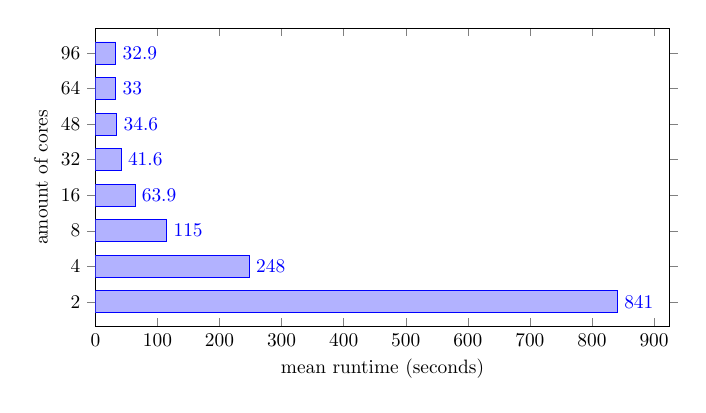
\begin{tikzpicture}[thick, scale=0.7]
		\begin{axis}[
			xbar, xmin=0,
			bar width=0.4cm,
			width=12cm, height=7cm, enlarge y limits=0.1,
			ylabel={amount of cores},
			xlabel={mean runtime (seconds)},
			symbolic y coords={2, 4, 8, 16, 32, 48, 64, 96},
			ytick=data,
			nodes near coords, nodes near coords align={horizontal},
			]
			\addplot coordinates {(841,2) (248,4) (115,8) (63.9,16) (41.6,32) (34.6,48) (33.0,64) (32.9,96)};
		\end{axis}
		\end{tikzpicture}
	}
%	\caption[Parallel Matrix Multiplication using Eden (two 1024x1024 matrices)]
%\end{figure}

\framebox{
	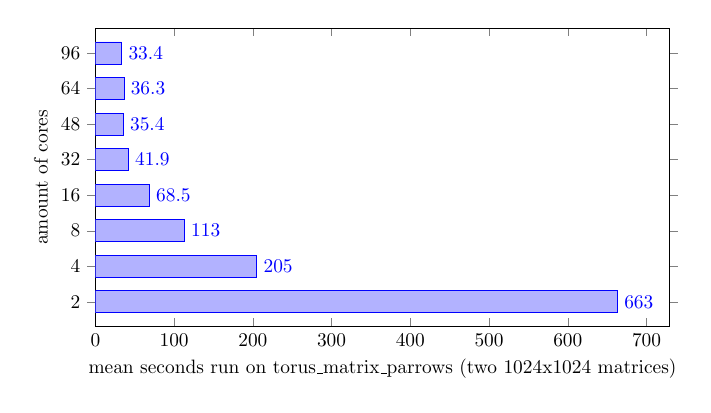
\begin{tikzpicture}[thick, scale=0.7]
	\begin{axis}[
	xbar, xmin=0,
	bar width=0.4cm,
	width=12cm, height=7cm, enlarge y limits=0.1,
	ylabel={amount of cores},
	xlabel={mean seconds run on torus\_matrix\_parrows (two 1024x1024 matrices)},
	symbolic y coords={2, 4, 8, 16, 32, 48, 64, 96},
	ytick=data,
	nodes near coords, nodes near coords align={horizontal},
	]
	\addplot coordinates {(663,2) (205,4) (113,8) (68.5,16) (41.9,32) (35.4,48) (36.3,64) (33.4,96)};
	\end{axis}
	\end{tikzpicture}
}

	%\pagebreak
	\section{Performance results}
\label{sec:benchmarks}

\newcommand{\rmtest}{Rabin--Miller test\xspace}
\newcommand{\sudokutest}{Sudoku\xspace}
\newcommand{\jacobitest}{Jacobi sum test\xspace}
\newcommand{\torustest}{Gentleman\xspace}
\newlength{\plotwidthSMP}
\setlength{\plotwidthSMP}{0.39\textwidth}
\newlength{\plotwidthDist}
\setlength{\plotwidthDist}{0.6\textwidth}


\newcommand{\performanceplot}[7]{
\begin{tikzpicture}
\begin{axis}[title={#1},
title style={align=center},
scale only axis, width=#7,
xlabel=Threads,
%xtick=data,
xtick distance=#4,
ylabel=Time (s),
ylabel near ticks,
minor tick num=2,
grid=major,
legend entries={#2},
legend style={at={(0.99,0.99)},anchor=north east},
max space between ticks=50pt,
grid style={line width=.1pt, draw=gray!10},
major grid style={line width=.2pt,draw=gray!50},
xmin=-1,
xmax=#6]
#5
\end{axis}
\end{tikzpicture}
}

\newcommand{\performancediffplot}[8]{
\begin{tikzpicture}
\begin{axis}[title={#1},
title style={align=center},
scale only axis, width=#8,
xlabel=Threads,
%xtick=data,
ytick distance=#6,
xtick distance=#4,
minor tick num=9,
ylabel=Absolute time difference (s),
ylabel near ticks,
grid=both,
legend entries={#2},
legend style={at={(0.99,0.99)},anchor=north east},
max space between ticks=50pt,
grid style={line width=.1pt, draw=gray!10},
major grid style={line width=.2pt,draw=gray!50},
xmin=-1,
xmax=#7]
#5
\end{axis}
\end{tikzpicture}
}

\newcommand{\speedupplot}[7]{
\begin{tikzpicture}
\begin{axis}[title={#1},
title style={align=center},
scale only axis, width=#7,
xlabel=Threads,
%xtick=data,
%ytick=data,
xtick distance=#4,
ytick distance=#4,
ylabel=Speedup,
ylabel near ticks,
grid=major,
legend entries={linear, #2},
legend style={at={(0.01,0.99)},anchor=north west},
max space between ticks=50pt,
grid style={line width=.1pt, draw=gray!10},
major grid style={line width=.2pt,draw=gray!50},
ymin=-1,
xmin=-1,
ymax=#6,
xmax=#6]
\addplot [domain=0:#3, no markers,dotted,thick]{x};
#5
\end{axis}
\end{tikzpicture}
}

\newcommand{\speedupdiffplot}[7]{
\begin{tikzpicture}
\begin{axis}[title={#1},
title style={align=center},
scale only axis, width=#7,
xlabel=Threads,
%xtick=data,
xtick distance=#4,
ytick distance=0.5,
ylabel=Absolute speedup difference,
ylabel near ticks,
grid=major,
legend entries={#2},
legend style={at={(0.99,0.99)},anchor=north east},
max space between ticks=50pt,
grid style={line width=.1pt, draw=gray!10},
major grid style={line width=.2pt,draw=gray!50},
xmin=-1,
xmax=#6]
#5
\end{axis}
\end{tikzpicture}
}

\subsection{Hardware}

We have tested our parallel DSL and algorithmic skeletons implemented
in it. Benchmarks were conducted both in a shared and in a distributed
memory setting. All benchmarks were done on the ``Glasgow grid'', consisting of
16 machines with 2 Intel\SymbReg~Xeon\SymbReg~E5-2640 v2 and 64 GB of DDR3 RAM each. Each processor has 8 cores and 16 (hyperthreaded) threads with a base frequency of 2 GHz and a turbo frequency of 2.50 GHz. This results in a total of 256 cores and 512 threads for the whole cluster. The operating system was Ubuntu 14.04 LTS with Kernel 3.19.0-33. Non-surprisingly, we found that hyperthreaded 32 cores do not behave in the same manner as real 16 cores (numbers here for a single machine). We disregarded the hyperthreading ability in most of the
cases.

We used a single node with 16 real cores as a shared memory testbed
and the whole grid with 256 real cores as a device to test our
distributed memory software.

\subsection{Test programs}

We used multiple tests that originated from different
sources. Most of them are parallel mathematical computations, initially
implemented in Eden. Table~\ref{tab:benches} summarizes.

\begin{table}
\caption{The benchmarks we use in this paper.}
\label{tab:benches}
\centering
%% something was wrong with separators in table
\renewcommand{\tabcolsep}{1em}
\begin{tabular}{lccll}
\toprule
Name & Area & Type & Origin & Citation \\
\midrule
\rmtest & Mathematics & |parMap+reduce| & Eden & \citet{Lobachev2012}\\
\jacobitest & Mathematics & |workpool+reduce| & Eden & \citet{Lobachev2012}\\
\torustest & Mathematics & |torus| & Eden & \citet{Eden:SkeletonBookChapter02}\\
\sudokutest & Puzzle & |parMap| & |Par| Monad & \citet{par-monad} 
\tablefootnote{actual code from: http://community.haskell.org/~simonmar/par-tutorial.pdf and https://github.com/simonmar/parconc-examples}\\
\bottomrule
\end{tabular}
\end{table}

\rmtest is a probabilistic primality test that iterates multiple (32--256 here)
``subtests''. Should a subtest fail, the input is definitely not a
prime. If all $n$ subtest pass, the input is composite with the
probability of $1/4^{n}$. 

Jacobi sum test or APRCL is also a primality test, that however,
guarantees the correctness of the result. It is probabilistic in the
sense that its run time is not certain. Unlike \rmtest, the subtests
of Jacobi sum test have very different durations. \citet{lobachev-phd}
\olcomment{discuss some optimisations of parallel APRCL.} Generic parallel
implementation of \rmtest and APRCL were presented in \citet{Lobachev2012}.

``Gentleman'' is a standard Eden test program, developed
for their |torus| skeleton. It implements a parallel matrix
multiplication \citep{Gentleman1978}. We ported an Eden based version \citep{Eden:SkeletonBookChapter02} to PArrows.

A~parallel Sudoku solver was used by \citet{par-monad} to compare |Par| Monad
to Multicore Haskell. We ported it to PArrows.



\subsection{What parallel Haskells run where}

The \ensuremath{\Conid{Par}} monad and Multicore Haskell can be executed on a shared
memory machines only. Although GpH is available on distributed memory
clusters, and newer distributed memory Haskells such as HdpH exist,
current support of distributed memory in PArrows is limited to
Eden. We used the MPI backend of Eden in a distributed memory
setting. However, for shared memory Eden features a ``CP'' backend
that merely copies the memory blocks between distributed heaps. In
this mode Eden still operates in the ``nothing shared'' setting, but
is adapted better to multicore machines. We label this version of Eden
in the plots as ``Eden~CP''.



\subsection{Effect of hyperthreading}

The PArrows version of \rmtest on a single node of the Glasgow grid
showed almost linear speedup (Fig.~\ref{fig:bench-rm-sm}). The speedup
of 64-task PArrows/Eden at 16 real cores version was 13.65, the
efficiency was 85.3\%.  However, if we increase the number of
requested cores to be 32---\ie if we use hyperthreading on 16 real
cores---the speedup does not increase that well. It is merely 15.99
for 32 tasks with PArrows/Eden. It is worse for other backends.  As
for 64 tasks, we obtain the speedup of 16.12 with PArrows/Eden at 32
hyperthreaded cores and only 13.55 with PArrows/Multicore
Haskell. Efficiency is 50.4\% and 42.3\%, respectively. The Eden
version used here was Eden~CP, the ``share nothing'' SMP build.

In the distributed memory setting the same effect ensues. We obtain
plummeting speedup of 124.31 at 512 hyperthreaded cores, whereas it was
213.172 for 256 real cores. Apparently, hyperthreading in the Glasgow
grid fails to execute two parallel Haskell processes with full-fledged
parallelism. For this reason, we did not regard hyperthreaded cores in
our speedup plots in Figs.~\ref{fig:bench-rm-sm}-\ref{fig:sudokuSMBenchmark}.


% rm 11213 32 32-sm speedup eden: 15.993037587283924
% -"- multi: 15.09948017762912
% -"- par: 14.909092857846693

% -"- 64 32-sm speedup eden: 16.118040224478424
% -"- multi: 13.545304115702333
% -"- par: 15.155709987503396

\subsection{Benchmark results}

The difference between, say, PArrows with |Par| Monad backend and a
genuine |Par|
Monad benchmark is very small. To give an example, it is ~0.4s in favour of PArrows for 16 cores (10.8s vs. 11.2s) and ~-0.8s in favour of the |Par| monad for 8 cores (16.1s vs. 16.9s) for
the Sudoku benchmark in the shared memory setting. It is almost invisible in speedup and
(non shown) run time plots. We thus show only the results for the
PArrows-enabled versions.

To show that PArrows induce very small overhead in a distributed context as well, we compare the original Eden
versions of the benchmark to its PArrows-enabled counterpart in the \rmtest, \torustest and \jacobitest benchmarks. We plot execution time differences between measurements for
PArrows and the corresponding backend in a separate plot
(Figs.~\ref{fig:bench-rm-dist}, \ref{fig:torusBenchmark}, \ref{fig:bench-jacobi-dist}). As an example, the differences range in
about 0.5~seconds for the execution time of 46~seconds on 256 cores
for distributed \rmtest with PArrows and Eden. For these comparisons, the plots show absolute
time differences that are not relative \wrt the total execution time.
Furthermore, the error bars ends were computed from pointwise maximum of both standard
deviations from both measurements for PArrows and non-PArrows
versions. These are the values provided by the |bench| package that we
used for benchmarking. We call a difference between two versions
significant when the border of the error bar of absolute time
difference is above or below zero. In other words: the time
difference is significant if it is above measurement error.

\subsubsection{\rmtest}\label{sec:rmtest}

\newcommand{\performanceSkelRMSM}[2]{
\performanceplot{Parallel run time of \rmtest ``#2''}{Eden CP, Multicore, |Par| Monad}{16}{4}{
\addplot+ [very thick] table [scatter, x="nCores", y="time", col sep=comma, mark=none,
smooth]{benchmarks/sm-rm/bench-sm-rm.bench.skelrm-parr-eden-cp-#1-#2.csv};
\addplot+ [very thick] table [scatter, x="nCores", y="time", col sep=comma, mark=none,
smooth]{benchmarks/sm-rm/bench-sm-rm.bench.skelrm-parr-mult-#1-#2.csv};
\addplot+ [very thick] table [scatter, x="nCores", y="time", col sep=comma, mark=none,
smooth]{benchmarks/sm-rm/bench-sm-rm.bench.skelrm-parr-par-#1-#2.csv};
}{17}{\plotwidthSMP}
}

\newcommand{\speedupSkelRMSM}[2]{
\speedupplot{Speedup of \rmtest ``#2''}{Eden CP, Multicore, |Par| Monad}{16}{4}{
\addplot+ [very thick] table [scatter, x="nCores", y="speedup", col sep=comma, mark=none,
smooth]{benchmarks/sm-rm/bench-sm-rm.bench.skelrm-parr-eden-cp-#1-#2.csv};
\addplot+ [very thick] table [scatter, x="nCores", y="speedup", col sep=comma, mark=none,
smooth]{benchmarks/sm-rm/bench-sm-rm.bench.skelrm-parr-mult-#1-#2.csv};
\addplot+ [very thick] table [scatter, x="nCores", y="speedup", col sep=comma, mark=none,
smooth]{benchmarks/sm-rm/bench-sm-rm.bench.skelrm-parr-par-#1-#2.csv};
}{17}{\plotwidthSMP}
}

\newcommand{\speedupSkelRMDist}[4]{
\speedupplot{Speedup of \rmtest ``#2''}{PArrows}{256}{#3}{
% \addplot [mark=*,very thick] table [scatter, x="nCores", y="speedup", col sep=comma, mark=none,
% smooth]{benchmarks/distributed-rm/bench-distributed.bench.skelrm-parrows-11213-#2.csv};
\addplot [mark=*,very thick,blue] table [scatter, x="nCores", y="speedup", col sep=comma, mark=none,
smooth]{benchmarks/distributed-rm/bench-distributed.bench.skelrm-parrows-#1-#2.csv};
% \addplot table [scatter, x="nCores", y="speedup", col sep=comma, mark=none,
% smooth]{benchmarks/distributed-rm/bench-distributed.bench.skelrm-eden-#1-#2.csv};
}{#4}{\plotwidthDist}
}

\newcommand{\performanceSkelRMDistDiff}[5]{
\performancediffplot{Run time differences\\for \rmtest ``#2''}{(Eden $-$ PArrows)}{256}{#3}{
\addplot+[mark=*,very thick,error bars/.cd,
    y dir=both,y explicit] table [x="nCores", y="time", y error="max stddev", col sep=comma, mark=dots,
smooth]{benchmarks/distributed-rm/#1-#2-diff.csv};
}{#4}{#5}{\plotwidthDist}
}

\begin{figure}
%\centering
%\performanceSkelRMSM{11213}{64}\hfill%
{\speedupSkelRMSM{11213}{32}}\hfill%
{\speedupSkelRMSM{11213}{64}}
\caption{Relative speedup of \rmtest on a multicore machine. We used the same PArrows-based implementation with
  different backends on the same hardware. Measurements were performed on a single node of the Glasgow
  grid; it has 16 real cores. Input was $2^{11213}-1$, we used 32 (left) or 64 (right)
  tasks. The
  closer to linear speedup the better.}
\label{fig:bench-rm-sm}
\end{figure}

\begin{figure}
\centering
%\performanceSkelRMDist{44497}{256}{32,64,128,256,512}{544}
%
{\speedupSkelRMDist{44497}{256}{32}{260}\label{subfig:rm-dist-a}}%
%\hfill%
{\performanceSkelRMDistDiff{44497}{256}{32}{0.5}{260}\label{subfig:rm-dist-b}}
\caption{Parallel performance of \rmtest on the Glasgow grid
  consisting of 256 cores. Input was $2^{44497}-1$, we used 256
  tasks. The top plot shows absolute speedup in a distributed memory setting. The
  closer to linear speedup the better. Time
  (and hence speedup) measurements for PArrows with Eden backend and
  Eden almost coincide. Hence, bottom plot shows
absolute time differences for this benchmark. The
higher the value, the better for PArrows\olcomment{CHECKME}.}
\label{fig:bench-rm-dist}
\end{figure}

\olcomment{THE ACTUAL TEXT IS MISSING. What do we see in the plots?
  Why is it good?}
The multicore version of our parallel \rmtest benchmark is depicted in
Figure~\ref{fig:bench-rm-sm}. We executed the test with 32 and 64
tasks. The plot shows the PArrows-enabled versions with corresponding backends.
The performance of PArrows/Eden~CP in shared memory is slightly better than
for SMP variants such as PArrows/Multicore Haskell and PArrows/|Par|
Monad but most of the time the performance is still comparable with the Multicore backend performing slightly worse than the other two in terms of speedup. In particular, the speedups for 16 cores fall behind quite noticeably with 11.69 for 32 tasks as Eden and the |Par| Monad both score 13.05 for 32 tasks. While the Multicore backend scores a bit better in the 64 tasks benchmark, its speedup of 12.70 is still behind the 13.65 and 13.33 of Eden and |Par| Monad, respectively.

Comparing the PArrows version of the \rmtest with the original from Eden with the MPI backend in a distributed memory setting, we see an almost linear speedup of
\rmtest with 256 tasks and input $2^{444497}-1$ in both versions. The sequential run time
was computed as the mean of three consecutive executions on a single
core---the single run took two hours 43 minutes. The zero difference  between
PArrows/Eden and Eden almost always lies on the error bar of
the measurement. The only exception, where the PArrows and Eden versions differ and it was it was significant, was for 64 cores, where it performed 0.49s better. This corresponds to
0.30\% relative time difference. Otherwise, PArrows was 0.23s (or 0.0007\%) slower for 32 cores, 0.26s (or 0.0030\%) slower for 128 cores, and 0.09s faster (or 0.0019\%) faster for 256 cores.

%As the PArrows version uses Eden in the backend, these numbers suggest that there is no real performance difference between using PArrows or Eden for this task as they trade blows in this benchmark. Additionally, PArrows with an Eden-based backend performing better than what it is based upon suggests that any difference in runtime between the two is more of an anomaly than a real difference.

\subsubsection{\jacobitest}

Continuing, the results of the \jacobitest in \ref{fig:bench-jacobi-dist} are as follows:

\newcommand{\speedupJacobiDist}[4]{
\speedupplot{Speedup of \jacobitest ``#2''}{PArrows}{256}{#3}{
% \addplot [mark=*,very thick] table [scatter, x="nCores", y="speedup", col sep=comma, mark=none,
% smooth]{benchmarks/distributed-rm/bench-distributed.bench.skelrm-parrows-11213-#2.csv};
\addplot [mark=*,very thick,blue] table [scatter, x="nCores", y="speedup", col sep=comma, mark=none,
smooth]{benchmarks/distributed-jacobi/bench-jacobi.bench.jacobi-parr-#1-#2.csv};
% \addplot table [scatter, x="nCores", y="speedup", col sep=comma, mark=none,
% smooth]{benchmarks/distributed-rm/bench-distributed.bench.skelrm-eden-#1-#2.csv};
}{#4}{\plotwidthDist}
}

\renewcommand{\speedupJacobiDist}[4]{
	\textcolor{red}{benchmark missing. in the works}
}

\newcommand{\performanceJacobiDistDiff}[5]{
\performancediffplot{Run time differences\\for \jacobitest ``#2''}{(Eden $-$ PArrows)}{256}{#3}{
\addplot+[mark=*,very thick,error bars/.cd,
    y dir=both,y explicit] table [x="nCores", y="time", y error="max stddev", col sep=comma, mark=dots,
smooth]{benchmarks/distributed-jacobi/#1-#2-diff.csv};
}{#4}{#5}{\plotwidthDist}
}

\renewcommand{\performanceJacobiDistDiff}[5]{
	\textcolor{red}{benchmark missing. in the works}
}

\begin{figure}
\centering
%\performanceSkelRMDist{44497}{256}{32,64,128,256,512}{544}
%
{\speedupJacobiDist{3}{1279}{32}{260}\label{subfig:rm-dist-a}}%
%\hfill%
{\performanceJacobiDistDiff{3}{1279}{32}{0.5}{260}\label{subfig:rm-dist-b}}
\caption{Parallel performance of \rmtest on the Glasgow grid
  consisting of 256 cores. Input was $2^{1279}-1$, we used 256
  tasks. The top plot shows absolute speedup in a distributed memory setting. The
  closer to linear speedup the better. Time
  (and hence speedup) measurements for PArrows with Eden backend and
  Eden almost coincide. Hence, bottom plot shows
absolute time differences for this benchmark. The
higher the value, the better for PArrows\olcomment{CHECKME}.}
\label{fig:bench-jacobi-dist}
\end{figure}

\mbcomment{FIXME: redo this test with $2^{44497}$}

\subsubsection{\torustest}

Next is the \torustest benchmark. The results of the comparison of vanilla Eden to our PArrows-based version can be found in \ref{fig:torusBenchmark}. While we do not see too much speedup for more than 16 cores, we can prove that the difference between the Eden and PArrows version are again marginal. The difference between PArrows and Eden is only significant for 16 and 64 cores where it ran 1.7\% and 2.7\% slower which corresponds to a real-time difference of 0.12s and 0.13s. For 256 cores PArrows performed 0.2\% slower which corresponds to 0.01s overhead.

\newcommand{\speedupTorusDist}[3]{
\speedupplot{Speedup of \torustest ``#1''}{PArrows}{256}{#2}{
\addplot [mark=*,very thick,blue] table [scatter, x="nCores", y="speedup", col sep=comma, mark=none,
smooth]{benchmarks/distributed-torus/bench-torus-distributed.bench.torus-matrix-parrows-#1.csv};
}{#3}{\plotwidthDist}
}

\renewcommand{\speedupTorusDist}[3]{
	\textcolor{red}{benchmark missing. in the works}
}


\newcommand{\performanceTorusDistDiff}[4]{
\performancediffplot{Run time differences\\for \torustest ``#1''}{(Eden $-$ PArrows)}{256}{#2}{
\addplot+[mark=*,very thick,error bars/.cd,
    y dir=both,y explicit] table [x="nCores", y="time", y error="max stddev", col sep=comma, mark=dots,
smooth]{benchmarks/distributed-torus/#1-diff.csv};
}{#3}{#4}{\plotwidthDist}
}

\renewcommand{\performanceTorusDistDiff}[4]{
		\textcolor{red}{benchmark missing. in the works}
}

\begin{figure}
\centering
%\performanceSkelRMDist{44497}{256}{32,64,128,256,512}{544}
%
{\speedupTorusDist{1024}{32}{260}\label{subfig:speedupTorusDist}}%
%\hfill%
{\performanceTorusDistDiff{1024}{32}{0.5}{260}\label{subfig:performancetorusDistDiff}}
\caption{Parallel performance of \torustest on the Glasgow grid
  consisting of 256 cores. Input was a matrix size of $1024$. The top plot shows absolute speedup in a distributed memory setting. The
  closer to linear speedup the better. Time
  (and hence speedup) measurements for PArrows with Eden backend and
  Eden almost coincide. Hence, bottom plot shows
absolute time differences for this benchmark. The
higher the value, the better for PArrows\olcomment{CHECKME}.}
\label{fig:torusBenchmark}
\end{figure}


\subsubsection{\sudokutest}

As the last Benchmark in this paper we present the \sudokutest in \ref{fig:sudokuSMBenchmark} running in a shared memory setting. Here we see all three SM backends performing similarly again like in the \rmtest SM benchmarks in Figs.~\ref{fig:sudokuSMBenchmark}-\ref{fig:sudokuSMBenchmark16000}. However, we notice that the Multicore backend seems to choke on a bigger input \ref{fig:sudokuSMBenchmark16000}. This is due to the benchmark only using |parMap| instead of a chunking variant (however we did not change that for simplicity's sake) and is reflected by debug output which shows, that of 16000 sparks being created (one for each sudoku) only 8365 were converted (executed) with the rest (7635) overflowing the runtime spark pool. Another remarkable finding is that the Eden backend seems to lack behind for $\leq$16 threads, but manages to pull ahead noticeably with all 32 threads of the system in use.


\newcommand{\performanceSudokuSM}[1]{
\performanceplot{Parallel run time of \sudokutest ``#1''}{Eden CP, Multicore, |Par| Monad}{16}{4}{
\addplot+ [very thick] table [scatter, x="nCores", y="time", col sep=comma, mark=none,
smooth]{benchmarks/sudoku-sm/bench-sudoku-sm.bench.parrows-sudoku-parmap-eden-sudoku17.#1.txt.csv};
\addplot+ [very thick] table [scatter, x="nCores", y="time", col sep=comma, mark=none,
smooth]{benchmarks/sudoku-sm/bench-sudoku-sm.bench.parrows-sudoku-parmap-mult-sudoku17.#1.txt.csv};
\addplot+ [very thick] table [scatter, x="nCores", y="time", col sep=comma, mark=none,
smooth]{benchmarks/sudoku-sm/bench-sudoku-sm.bench.parrows-sudoku-parmap-par-sudoku17.#1.txt.csv};
%\addplot+ [very thick] table [scatter, x="nCores", y="time", col sep=comma, mark=none,
%smooth]{benchmarks/sudoku-sm/bench-sudoku-sm.bench.parmonad-sudoku-sudoku17.#1.txt.csv};
}{17}{\plotwidthSMP}
}

\newcommand{\speedupSudokuSM}[1]{
\speedupplot{ Parallel speedup of \sudokutest ``#1''}{Eden CP, Multicore, |Par| Monad}{16}{4}{
\addplot+ [very thick] table [scatter, x="nCores", y="speedup", col sep=comma, mark=none,
smooth]{benchmarks/sudoku-sm/bench-sudoku-sm.bench.parrows-sudoku-parmap-eden-sudoku17.#1.txt.csv};
\addplot+ [very thick] table [scatter, x="nCores", y="speedup", col sep=comma, mark=none,
smooth]{benchmarks/sudoku-sm/bench-sudoku-sm.bench.parrows-sudoku-parmap-mult-sudoku17.#1.txt.csv};
\addplot+ [very thick] table [scatter, x="nCores", y="speedup", col sep=comma, mark=none,
smooth]{benchmarks/sudoku-sm/bench-sudoku-sm.bench.parrows-sudoku-parmap-par-sudoku17.#1.txt.csv};
%\addplot+ [very thick] table [scatter, x="nCores", y="speedup", col sep=comma, mark=none,
%smooth]{benchmarks/sudoku-sm/bench-sudoku-sm.bench.parmonad-sudoku-sudoku17.#1.txt.csv};
}{17}{\plotwidthSMP}
}

\begin{figure}
\centering
%\performanceSkelRMDist{44497}{256}{32,64,128,256,512}{544}
%
{\speedupSudokuSM{1000}\label{subfig:speedupSudokuSM}}%
%\hfill%
{\performanceSudokuSM{1000}\label{subfig:performanceSudokuSM}}
\caption{Relative speedup of \sudokutest on a multicore machine. We used the same PArrows-based implementation with
  different backends on the same hardware and the |parMap| version from the |Par| Monad examples. Measurements were performed on a single node of the Glasgow
  grid; it has 16 real cores and 32 threads. Input was a file of $1000$ Sudokus. The
  closer to linear speedup the better.}
\label{fig:sudokuSMBenchmark}
\end{figure}

\begin{figure}
\centering
%\performanceSkelRMDist{44497}{256}{32,64,128,256,512}{544}
%
{\speedupSudokuSM{16000}\label{subfig:speedupSudokuSM16000}}%
%\hfill%
{\performanceSudokuSM{16000}\label{subfig:performanceSudokuSM16000}}
\caption{Relative speedup of \sudokutest on a multicore machine. We used the same PArrows-based implementation with
  different backends on the same hardware and the |parMap| version from the |Par| Monad examples. Measurements were performed on a single node of the Glasgow
  grid; it has 16 real cores and 32 threads. Input was a file of $16000$ Sudokus. The
  closer to linear speedup the better. The Multicore version shows signs of choking with too many sparks being created.}
\label{fig:sudokuSMBenchmark16000}
\end{figure}

	%%\pagebreak
	\section{Conclusion}
As we have seen in this paper, arrows are a useful tool for composing parallel programs. We have already seen that they have some benefits over existing parallel Haskells as they are, by nature, more extensible. Performancewise, parallel arrows are on par with existing parallel Haskells, as they do not introduce any notable overhead. While we have seen that the parallel arrows can express computation on clusters, it is noteworthy that in its current state, the parallel arrow API doesn't have as much control over data-flow as for example Eden. In its current state this will end up in the root node being a possible bottleneck on clusters when parallel arrows are combined with \code{>>>}. This can probably be remedied by introducing some sort of a Java-like Future construct that can be passed between nodes so that nodes can communicate without going through the root node. This will have to be implemented in a follow up paper, though.
	%\pagebreak
        \bibliographystyle{abbrvnat}
	\bibliography{references,main}
        \appendix
	\section{Utility Arrows}\label{utilfns}
Following are definitions of some utility Arrows used in this paper that have been lef out for brevity.
We start with the |second| combinator from \citet{HughesArrows}, which is a mirrored version of |first|, which is for example used in the definition of |***|: 
\begin{code}
second :: Arrow arr => arr a b -> arr (c, a) (c, b)
second f = arr swap >>> first f >>> arr swap
	where swap (x, y) = (y, x)
\end{code}

Next, we also define |map|, |foldl| and |zipWith| on Arrows.
The |mapArr| combinator (Fig.~\ref{fig:mapArr}) lifts any arrow |arr a
b| to an arrow |arr [a] [b]| \cite{programming_with_arrows}. 
Similarly, we can also define |foldlArr| (Fig.~\ref{fig:foldlArr}) that lifts any arrow |arr (b, a) b| with a neutral element |b| to |arr [a] b|.

\begin{figure}[h]
\begin{code}
mapArr :: ArrowChoice arr => arr a b -> arr [a] [b]
mapArr f =
	arr listcase >>>
	arr (const []) ||| (f *** mapArr f >>> arr (uncurry (:)))

listcase [] = Left ()
listcase (x:xs) = Right (x,xs)
\end{code}
\caption{The definition of |map| over Arrows and the |listcase| helper
function.}
\label{fig:mapArr}
\end{figure}

\begin{figure}[h]
\begin{code}
foldlArr :: (ArrowChoice arr, ArrowApply arr) => arr (b, a) b -> b -> arr [a] b
foldlArr f b =
	arr listcase >>>
	arr (const b) |||
		(first (arr (\a -> (b, a)) >>> f >>> arr (foldlArr f)) >>> app)
\end{code}
\caption{The definition of |foldl| over Arrows.}
\label{fig:foldlArr}
\end{figure}

Finally, with the help of |mapArr| (Fig.~\ref{fig:mapArr}), we can define |zipWithArr|  (Fig.~\ref{fig:zipWithArr}) that lifts any arrow |arr (a, b) c| to an arrow |arr ([a], [b]) [c]|.
\begin{figure}[h]
\begin{code}
zipWithArr :: ArrowChoice arr => arr (a, b) c -> arr ([a], [b]) [c]
zipWithArr f = (arr $ \(as, bs) -> zipWith (,) as bs) >>> mapArr f
\end{code}
\caption{|zipWith| over arrows.}
\label{fig:zipWithArr}
\end{figure}
 %$ %% formatting

These combinators make use of the |ArrowChoice| type class which provides the |pipepipepipe| combinator. It takes two arrows |arr a c| and |arr b c| and combines them into a new arrow |arr (Either a b) c| which pipes all |Left a|'s to the first arrow and all |Right b|'s to the second arrow:
% \begin{figure}[htb]
\begin{code}
(pipepipepipe) :: ArrowChoice arr a c -> arr b c -> arr (Either a b) c
\end{code}
% \caption{Type signature of \pipepipepipe}
% \label{fig:codeSigPipePipePipe}
% \end{figure}

With the zipWithArr combinator we can also write a combinator |listApp|, that lifts a list of arrows |[arr a b]| to an arrow |arr [a] [b]|.
% \begin{figure}[htb]
\begin{code}
listApp :: (ArrowChoice arr, ArrowApply arr) => [arr a b] -> arr [a] [b]
listApp fs = (arr $ \as -> (fs, as)) >>> zipWithArr app
\end{code}
% \caption{Definition of |listApp|}
% \label{fig:listApp}
% \end{figure}
% $ %% formatting
Note that  this additionally makes use of the |ArrowApply| typeclass that allows us to evaluate arrows with |app :: arr (arr a b, a) c|.

% $ %% formatting

\section{Omitted Function Definitions}
\label{app:omitted}
We have omitted some function definitions in the main text for
brevity, and redeem this here.

To begin with, we give the actual implementation of the non-configurable instance of the |ArrowParallel| instance:

\begin{figure}
\begin{code}
instance (NFData b, ArrowApply arr, ArrowChoice arr) => ArrowParallel arr a b () where
    parEvalN _ fs = parEvalN (hack fs) fs
                    where
                        hack :: (NFData b) => [arr a b] -> Conf b
                        hack _ = Conf rdeepseq
\end{code}
\caption{The actual default implementation of GpH's |ArrowParallel|.}
\label{fig:actualNonConfigMulticore}
\end{figure}

%
Next, we warp Eden's build-in Futures in PArrows as in
Figure~\ref{fig:RDFuture}, where |rd| is the accessor function for the |RD| wrapped inside |RemoteData|. Furthermore, in order for these |Future| types to fit with the |ArrowParallel| instances we gave earlier, we have to give the necessary |NFData| and |Trans| instances, the latter are only needed in Eden. The |Trans| instance does not have any functions declared as the default implementation suffices here. Furthermore, because |MVar| already ships with a |NFData| instance, we only have to supply a simple delegating |NFData| instance for our |RemoteData| type, where |rd| simply unwraps |RD|. The |Trans| instance does not have any functions declared as the default implementation suffices:

% \begin{figure}[h]
\begin{code}
instance NFData (RemoteData a) where
    rnf = rnf . rd
instance Trans (RemoteData a)
\end{code}
% \caption{NFData and Trans instances for the RemoteData type. The Trans instance does not have any functions declared as the default implementation suffices here. See \url{https://hackage.haskell.org/package/edenmodules-1.2.0.0/docs/Control-Parallel-Eden.html\#g:5} for more information.}
% \end{figure}

\begin{figure}[thb]
%parMap
\includegraphics[scale=0.7]{images/parMap}
\caption{Schematic depiction of |parMap|.}
\label{fig:parMapImg}

\begin{code}
parMap :: (ArrowParallel arr a b conf) => conf -> (arr a b) -> (arr [a] [b])
parMap conf f = parEvalN conf (repeat f)
\end{code}
\caption{Definition of parMap.}
\label{fig:parMap}

%parMapStream
\includegraphics[scale=0.7]{images/parMapStream}
\caption{Schematic depiction of |parMapStream|.}
\label{fig:parMapStreamImg}

\begin{code}
parMapStream :: (ArrowParallel arr a b conf, ArrowChoice arr, ArrowApply arr) =>
	conf -> ChunkSize -> arr a b -> arr [a] [b]
parMapStream conf chunkSize f = parEvalNLazy conf chunkSize (repeat f)
\end{code}
\caption{Definition of |parMapStream|.}
\label{fig:parMapStream}
\end{figure}

Figures~\ref{fig:parMapImg}--\ref{fig:parMapStream} show the definitions and a visualizations of two parallel |map| variants, defined using |parEvalN| and its lazy counterpart.

Arrow versions of Eden's |shuffle|, |unshuffle| and the definition of |takeEach| are in Figure~\ref{fig:edenshuffleetc}. Similarly, Figure~\ref{fig:edenlazyrightrotate} contains the definition of arrow versions of Eden's |lazy| and |rightRotate| utility functions. Fig.~\ref{fig:lazyzip3etc} contains Eden's definition of |lazyzip3| together with the utility functions |uncurry3| and |threetotwo|.
The full definition of |farmChunk| is in Figure~\ref{fig:farmChunk}.
Eden definition of |ring| skeleton is in Figure~\ref{fig:ringEden}. It
follows \citet{Loogen2012}.


\begin{figure}[h]
\begin{code}
data RemoteData a = RD { rd :: RD a }

instance (Trans a) => Future RemoteData a where
    put = arr (\a -> RD { rd = release a })
    get = arr rd >>> arr fetch
\end{code}
\caption{|RD|-based |RemoteData| version of |Future| for the Eden backend.}
\label{fig:RDFuture}
\end{figure}

\begin{figure}[h]
\begin{code}
shuffle :: (Arrow arr) => arr [[a]] [a]
shuffle = arr (concat . transpose)

unshuffle :: (Arrow arr) => Int -> arr [a] [[a]]
unshuffle n = arr (\xs -> [takeEach n (drop i xs) | i <- [0..n-1]])

takeEach :: Int -> [a] -> [a]
takeEach n [] = []
takeEach n (x:xs) = x : takeEach n (drop (n-1) xs)
\end{code}
\caption{Definitions of |shuffle|, |unshuffle|, |takeEach|.}
\label{fig:edenshuffleetc}
\end{figure}

\begin{figure}[h]
\begin{code}
lazy :: (Arrow arr) => arr [a] [a]
lazy = arr (\ ~(x:xs) -> x : lazy xs)

rightRotate :: (Arrow arr) => arr [a] [a]
rightRotate = arr $ \list -> case list of
  [] -> []
  xs -> last xs : init xs
\end{code}
\caption{Definitions of |lazy| and |rightRotate|.}
\label{fig:edenlazyrightrotate}
\end{figure}

\begin{figure}[h]
\begin{code}
lazyzip3 :: [a] -> [b] -> [c] -> [(a, b, c)]
lazyzip3 as bs cs = zip3 as (lazy bs) (lazy cs)

uncurry3 :: (a -> b -> c -> d) -> (a, (b, c)) -> d
uncurry3 f (a, (b, c)) = f a b c

threetotwo :: (Arrow arr) => arr (a, b, c) (a, (b, c))
threetotwo = arr $ \ ~(a, b, c) -> (a, (b, c))
\end{code}
\caption{Definitions of |lazyzip3|, |uncurry3| and |threetotwo|.}
\label{fig:lazyzip3etc}
\end{figure}

\begin{figure}[h]
\begin{code}
farmChunk :: (ArrowParallel arr a b conf, ArrowParallel arr [a] [b] conf, 
             ArrowChoice arr, ArrowApply arr) =>
	conf -> ChunkSize -> NumCores -> arr a b -> arr [a] [b]
farmChunk conf chunkSize numCores f =
	unshuffle numCores >>>
	parEvalNLazy conf chunkSize (repeat (mapArr f)) >>>
	shuffle
\end{code}
\caption{Definition of |farmChunk|.}
\label{fig:farmChunk}
\end{figure}

\begin{figure}[h]
\begin{code}
ringSimple :: (Trans i, Trans o, Trans r) => (i -> r -> (o,r)) -> [i] -> [o]
ringSimple f is =  os
  where (os,ringOuts) = unzip (parMap (toRD $ uncurry f) (zip is $ lazy ringIns))
        ringIns = rightRotate ringOuts

toRD :: (Trans i, Trans o, Trans r) => ((i,r) -> (o,r)) -> ((i, RD r) -> (o, RD r))
toRD  f (i, ringIn)  = (o, release ringOut)
  where (o, ringOut) = f (i, fetch ringIn)

rightRotate    :: [a] -> [a]
rightRotate [] =  []
rightRotate xs =  last xs : init xs

lazy :: [a] -> [a]
lazy ~(x:xs) = x : lazy xs
\end{code}
\caption{Eden's definition of the |ring| skeleton.}
\label{fig:ringEden}
\end{figure}

The |parEval2| skeleton is defined in Figure~\ref{fig:parEval2}. 
We start by transforming the |(a, c)| input into a two-element list |[Either a c]| by first tagging the two inputs with |Left| and |Right| and wrapping the right element in a singleton list with |return| so that we can combine them with |arr (uncurry (:))|. Next, we feed this list into a parallel arrow running on two instances of |f +++ g| as described above. After the calculation is finished, we convert the resulting |[Either b d]| into |([b], [d])| with |arr partitionEithers|. The two lists in this tuple contain only one element each by construction, so we can finally just convert the tuple to |(b, d)| in the last step.
\begin{figure}[h]
\begin{code}
parEval2 :: (ArrowChoice arr,
	ArrowParallel arr (Either a c) (Either b d) conf) =>
	conf -> arr a b -> arr c d -> arr (a, c) (b, d)
parEval2 conf f g =
	arr Left *** (arr Right >>> arr return) >>>
	arr (uncurry (:)) >>>
	parEvalN conf (replicate 2 (f +++ g)) >>>
	arr partitionEithers >>>
	arr head *** arr head
\end{code}
	\caption{Definition of |parEval2|.}
	\label{fig:parEval2}
\end{figure}
Furthermore, Fig.~\ref{fig:torus_example_rest} contains the ommited definitions of |prMMTr| (which calculates $AB^T$ for two matrices $A$ and $B$), |splitMatrix| (which splits the a matrix into chunks), and lastly |matAdd|, that calculates $A + B$ for two matrices $A$ and $B$.
\begin{figure}[h]
\begin{code}
prMMTr m1 m2 = [[sum (zipWith (*) row col) | col <- m2 ] | row <- m1]

splitMatrix :: Int -> Matrix -> [[Matrix]]
splitMatrix size matrix = map (transpose . map (chunksOf size)) $ chunksOf size $ matrix

matAdd = chunksOf (dimX x) $ zipWith (+) (concat x) (concat y)
\end{code}
	\caption{Definition of |prMMTr|, |splitMatrix| and |matAdd|.}
	\label{fig:torus_example_rest}
\end{figure}

\section{Syntactic Sugar} \label{syntacticSugar}
Finally, we also give the definitions for some syntactic sugar for PArrows, namely |***| and |&&&|.
For basic arrows, we have the |***| combinator (Fig.~\ref{fig:syntacticSugarArrows}) which allows us to combine two arrows |arr a b| and |arr c d| into an arrow |arr (a, c) (b, d)| which does both computations at once. This can easily be translated into a parallel version |***| with the use of |parEval2|, but for this we require a backend which has an implementation that does not require any configuration (hence the |()| as the |conf| parameter% in Fig.~\ref{fig:par***}
):
% \begin{figure}[h]
\begin{code}
(|***|) :: (ArrowChoice arr, ArrowParallel arr (Either a c) (Either b d) ())) =>
	arr a b -> arr c d -> arr (a, c) (b, d)
(|***|) = parEval2 ()
\end{code}
% \caption{Definition of |parstar|, the parallel version of |***|.}
% \label{fig:par***}
% \end{figure}
% With this we can analogously to the serial |&&&|
We define the parallel |&&&| % (Fig.~\ref{fig:par&&&}) 
in a similar manner to its sequential pendant |&&&| (Fig.~\ref{fig:syntacticSugarArrows}):
% \begin{figure}[h]
\begin{code}
(|&&&|) :: (ArrowChoice arr, ArrowParallel arr (Either a a) (Either b c) ()) =>
	arr a b -> arr a c -> arr a (b, c)
(|&&&|) f g = (arr $ \a -> (a, a)) >>> f |***| g
\end{code} % $ %% formatting
% \caption{Definition of |parand| - the parallel version of |&&&|.}
% \label{fig:par&&&}
% \end{figure}


%%% Local Variables:
%%% mode: latex
%%% TeX-master: "main"
%%% End:

\end{document}